\section{Evaluation}
\label{sec:evaluation}

\begin{enumerate}
    \item Benchmarks (describe our benchmarks)
    \item Results (total time, split out SMPT time from our rust code time)
    \item Analysis of optimizations (how much time they save, petri net sizes, semilinear set sizes)
    \item Limitations (examples we cannot solve, future work that would help)
\end{enumerate}


\noindent
\textbf{Experimental Setup.}
All experiments ran on a second generation Lenovo Notebook ThinkPad P16s, with 16 AMD cores and a RAM of 58 GB, with a Linux Ubuntu 24.04.2 operating system.
%
We plan on making all our code, benchmarks raw results publicly available with the final version of this paper.
 


\subsection{Benchmarks Overview}
\label{subsec:benchmarks}

\begin{itemize}
	\item \textbf{Core expressions \& multi request workflows}: Benchmarks testing arithmetic, boolean, and simple control expression.
	\item \textbf{Fred (mixed arithmetic)}: Mixed control and arithmetic transformations (Fred series).
	\item \textbf{Stop (circular-increment) series}: Circular increment loops and variants.
	\item \textbf{Concurrency \& locking loops}: Concurrent looping patterns with locking and tricky interactions.
	\item \textbf{Non-deterministic choice \& randomness}: Random choice and non-deterministic branching benchmarks.
	\item \textbf{Networking \& system protocols}: Networking protocols and system-level monitoring.
	\item \textbf{JSON state-machine examples}: Example JSON-encoded state machine workflows.
\end{itemize}


\subsection{Results}



\begin{table}[H]
	\centering
	% Load the tabular from the external file:
	\begin{table}[H]
	\centering
	\small
	% increase horizontal padding between columns
	\setlength{\tabcolsep}{5pt}
	\renewcommand{\arraystretch}{0.9}
	\begin{tabular*}{\textwidth}{@{\extracolsep{\fill}}%
			p{1.5cm}   % Category
			p{1.0cm} % Benchmark
			c        % Serializable
			c c c c c c % Features
			r r       % Cert, Total
		}
		\toprule
		\multicolumn{2}{c}{\textbf{Benchmark}}
		& \textbf{Serializable}
		& \multicolumn{6}{c}{\textbf{Features}}
		& \multicolumn{2}{c}{\textbf{Runtime (ms)}} \\
		\cmidrule(lr){1-2} \cmidrule(lr){3-3} \cmidrule(lr){4-9} \cmidrule(lr){10-11}
		&
		&
		& If & While & \texttt{?} & Arith & Yield & Multi-req
		& Cert. & Total \\
		\midrule
		\multirow{7}{=}{Core expressions} & \texttt{a1.ser} & \greencmark &  & \cmark &  &  &       &   & 2 & 47 \\
		 & \texttt{a2.ser} & \xmark &  &        &  &  & \cmark &   & 280 & 296 \\
		 & \texttt{a3.ser} & \greencmark &  &        &  &  &       &   & 1 & 32 \\
		 & \texttt{a4.ser} & \greencmark &  &        &  &  & \cmark & \cmark & 637 & 1071 \\
		 & \texttt{a5.ser} & \greencmark &  & \cmark &  &  & \cmark & \cmark & 3234 & 13624 \\
		 & \texttt{a6.ser} & \xmark &  &        &  &  & \cmark & \cmark & 757 & 775 \\
		 & \texttt{a7.ser} & \greencmark & \cmark & \cmark &  &  & \cmark &   & 4 & 33 \\
		\midrule
		\multirow{4}{=}{State machines} & \texttt{b1.json} & \greencmark & \cmark &        &  &  & \cmark & \cmark & 683 & 968 \\
		 & \texttt{b2.json} & \greencmark & \cmark &        &  &  & \cmark & \cmark & 2063 & 7802 \\
		 & \texttt{b3.json} & \greencmark & \cmark &        &  &  & \cmark & \cmark & 730 & 2080 \\
		 & \texttt{b4.json} & \greencmark & \cmark &        &  &  & \cmark & \cmark & 660 & 1909 \\
		\midrule
		\multirow{8}{=}{Fred (mixed arithmetic)} & \texttt{c1.ser} & \xmark &  & \cmark &  & \cmark & \cmark & \cmark & 356195 & 356299 \\
		 & \texttt{c2.ser} & \greencmark &  & \cmark &  & \cmark & \cmark & \cmark & 9858 & 292228 \\
		 & \texttt{c3.ser} & \greencmark &  & \cmark &  & \cmark & \cmark & \cmark & 1886 & 2397 \\
		 & \texttt{c4.ser} & \greencmark &  & \cmark &  & \cmark & \cmark & \cmark & 4336 & 7193 \\
		 & \texttt{c5.ser} & \xmark &  & \cmark &  & \cmark & \cmark & \cmark & 43694 & 43735 \\
		 & \texttt{c6.ser} & \xmark &  & \cmark &  & \cmark & \cmark & \cmark & 629 & 698 \\
		 & \texttt{c7.ser} & \xmark &  & \cmark &  & \cmark & \cmark & \cmark & 797 & 875 \\
		 & \texttt{c8.ser} & \greencmark &  & \cmark &  & \cmark & \cmark & \cmark & 4357 & 8931 \\
		\midrule
		\multirow{5}{=}{Circular increment} & \texttt{d1.ser} & \greencmark & \cmark & \cmark & \cmark &  & \cmark &   & 2391 & 5373 \\
		 & \texttt{d2.ser} & \xmark & \cmark &        & \cmark &  &   \cmark &   & 628 & 731 \\
		 & \texttt{d3.ser} & \greencmark & \cmark & \cmark & \cmark &  &  \cmark &   & 2642 & 10266 \\
		 & \texttt{d4.ser} & \greencmark & \cmark & \cmark & \cmark &  &     \cmark &   & 5604 & 22249 \\
		 & \texttt{d5.ser} & \xmark & \cmark &        &  &  & \cmark &   & 495 & 554 \\
		\midrule
		\multirow{7}{=}{Concurrency \& locking loops} & \texttt{e1.ser} & \greencmark &  & \cmark &  &  & \cmark &   & 351 & 502 \\
		 & \texttt{e2.ser} & \xmark & \cmark & \cmark &  & \cmark & \cmark & \cmark & \texttt{TIMEOUT} & \texttt{TIMEOUT} \\
		 & \texttt{e3.ser} & \xmark & \cmark & \cmark &  & \cmark &   \cmark & \cmark & 24899 & 25039 \\
		 & \texttt{e4.ser} & \xmark & \cmark & \cmark &  &  \cmark &   \cmark & \cmark & 273062 & 273351 \\
		 & \texttt{e5.ser} & \greencmark & \cmark & \cmark & \cmark &  & \cmark &   & 2 & 55 \\
		 & \texttt{e6.ser} & \greencmark & \cmark & \cmark & \cmark &  & \cmark &   & 10 & 114 \\
		 & \texttt{e7.ser} & \greencmark &  & \cmark &  &  &   \cmark &   & 299 & 444 \\
		\midrule
		\multirow{9}{=}{Non-deterministic \& randomness} & \texttt{f1.ser} & \greencmark & \cmark &    \cmark    & \cmark &  & \cmark &   & 388 & 494 \\
		 & \texttt{f2.ser} & \xmark & \cmark &   \cmark     & \cmark &  & \cmark &   & 612 & 676 \\
		 & \texttt{f3.ser} & \xmark &  &        &  & \cmark &   \cmark & \cmark & 653 & 716 \\
		 & \texttt{f4.ser} & \greencmark &  &     \cmark   &  & \cmark & \cmark & \cmark & 1626 & 9515 \\
		 & \texttt{f5.ser} & \greencmark & \cmark &        & \cmark &  &       &   & 7401 & 11301 \\
		 & \texttt{f6.ser} & \xmark & \cmark &        & \cmark &  & \cmark &   & 646 & 830 \\
		 & \texttt{f7.ser} & \xmark & \cmark &        & \cmark &  &  \cmark &   & 400 & 427 \\
		 & \texttt{f8.ser} & \xmark & \cmark &        & \cmark &  &   \cmark &   & 773 & 802 \\
		 & \texttt{f9.ser} & \greencmark & \cmark &        & \cmark &  &  \cmark &   & 10 & 94 \\
		\midrule
		\multirow{7}{=}{Networking \& system protocols} & \texttt{g1.ser} & \xmark & \cmark & \cmark &  & \cmark & \cmark & \cmark & 59312 & 74539 \\
		 & \texttt{g2.ser} & \greencmark & \cmark & \cmark &  & \cmark & \cmark & \cmark & \texttt{TIMEOUT} & \texttt{TIMEOUT} \\
		 & \texttt{g3.ser} & \xmark & \cmark & \cmark & \cmark & \cmark & \cmark & \cmark & 20557 & 20954 \\
		 & \texttt{g4.ser} & \xmark & \cmark & \cmark & \cmark & \cmark & \cmark & \cmark & 6859 & 7047 \\
		 & \texttt{g5.ser} & \greencmark & \cmark & \cmark & \cmark & \cmark &   \cmark & \cmark & 3047 & 12324 \\
		 & \texttt{g6.ser} & \xmark & \cmark &        & \cmark & \cmark & \cmark &   & 8193 & 8285 \\
		 & \texttt{g7.ser} & \greencmark & \cmark &        & \cmark & \cmark &       &   & 6886 & 252752 \\
		\midrule
\bottomrule
	\end{tabular*}
\end{table}

	\caption{Overview of benchmarks with combined categories and updated serializability markings. All optimizations were used, as well as a timeout value of 500 seconds.}
\label{tab:benchmarks-all}
\end{table}


\subsection{Optimization Analysis}


%\begin{figure}[htbp]
%	\centering
%	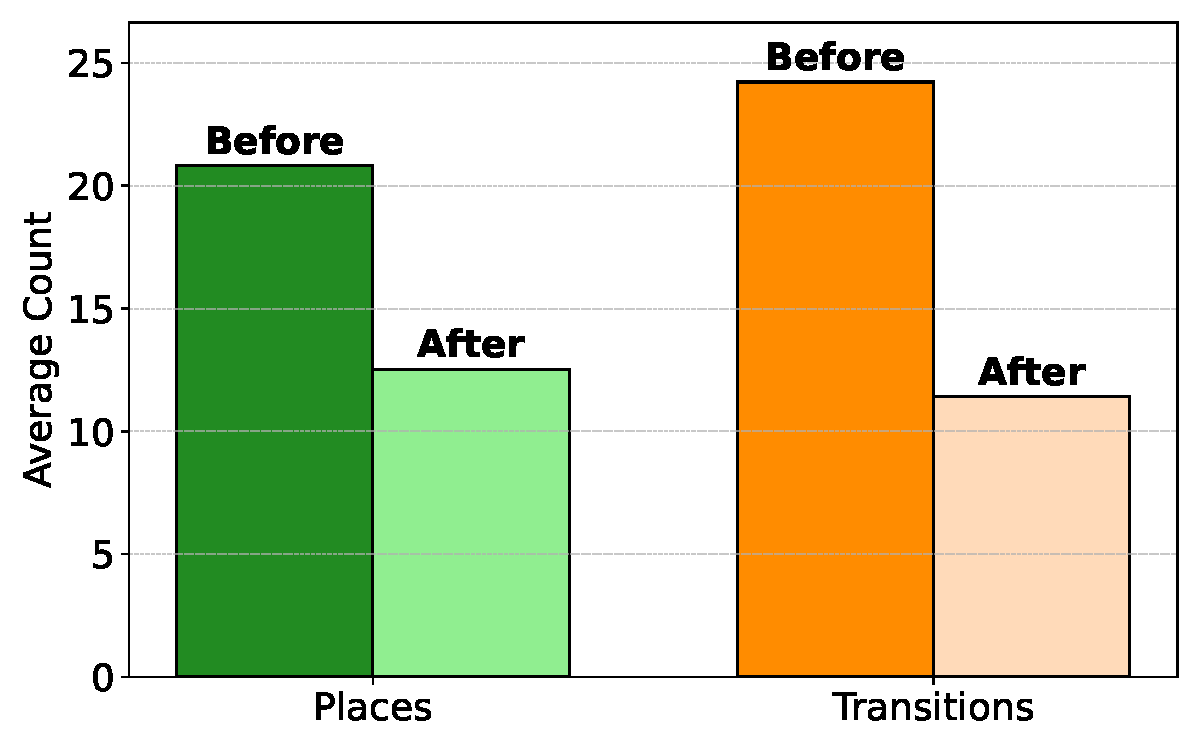
\includegraphics[width=0.4\textwidth]{plots/petri_size_reduction_plot.pdf}
%	\caption{Size reduction of Petri nets through optimization techniques. The plot shows the reduction in the number of places and transitions after applying our optimization passes. Averaged on all Petri Nets of 50 benchmarks (timeout 30 seconds).}
%	\label{fig:petri_size_reduction}
%\end{figure}


%\begin{figure}[htbp]
%	\centering
%	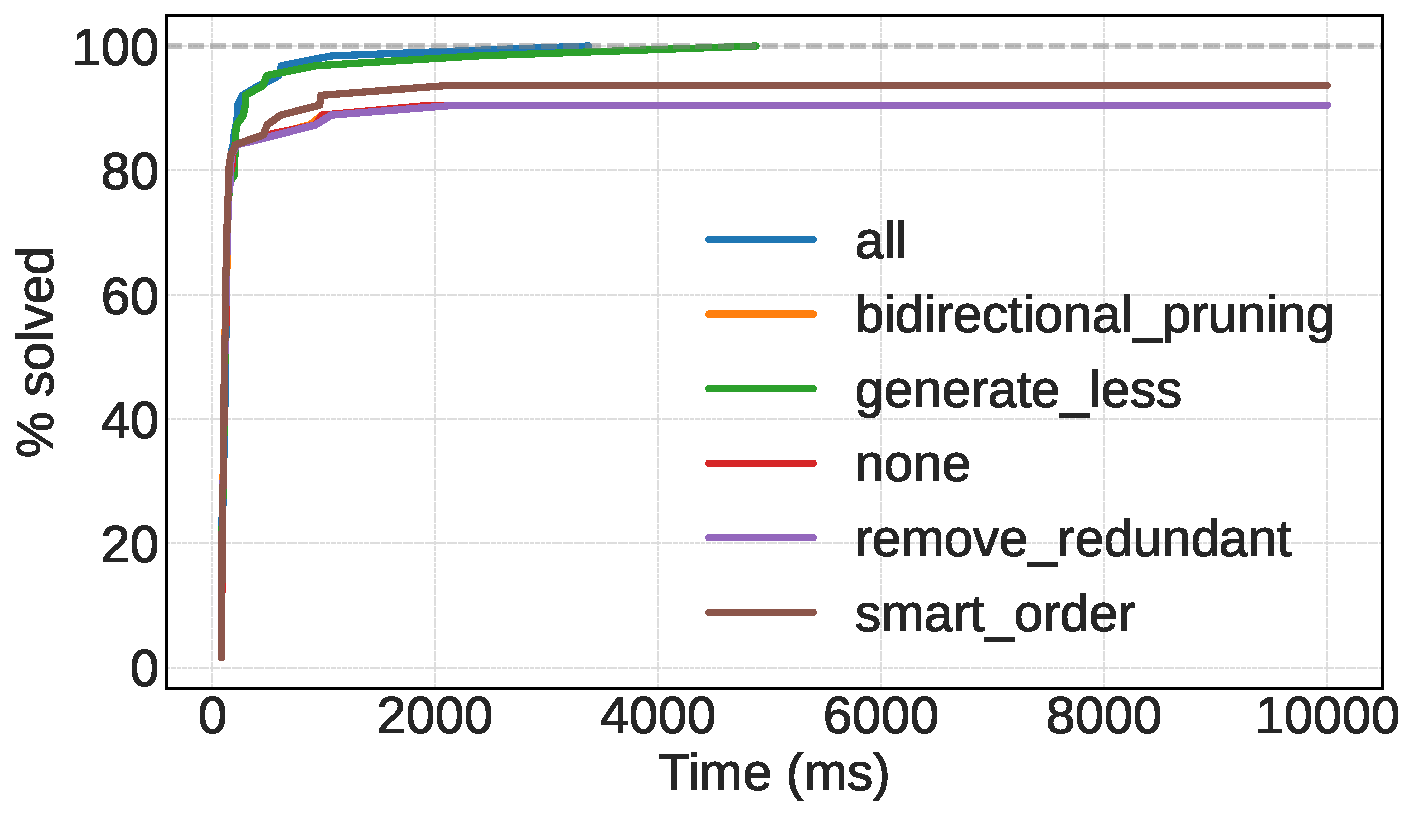
\includegraphics[width=0.4\textwidth]{plots/timeout_10000_cumulative_solved_linear.pdf}
%	\caption{Size reduction of Petri nets through optimization techniques. The plot shows the reduction in the number of places and transitions after applying our optimization passes. Averaged on all Petri Nets of 50 benchmarks (timeout 30 seconds).}
%	\label{fig:runtime}
%\end{figure}



\begin{center}
		\begin{minipage}[t]{0.48\textwidth}
		\centering
		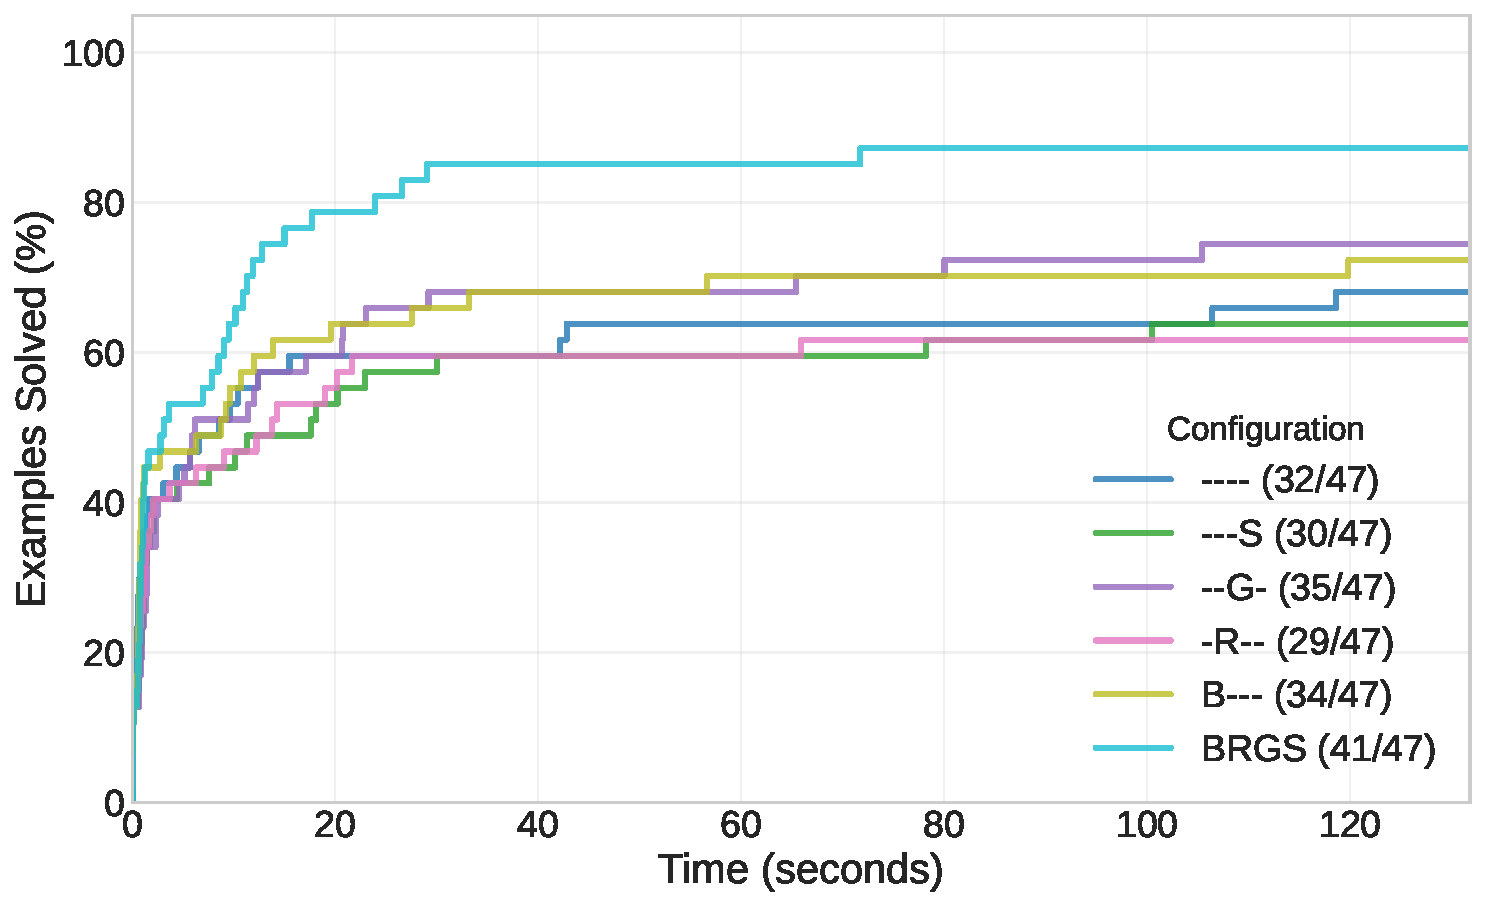
\includegraphics[width=\linewidth]{figures/cactus_plot.pdf}
		\captionof{figure}{Cumulative number of solved instances over time with a 150-second timeout.}
		\label{fig:timeout_cumulative_solved_log}
	\end{minipage}\hfill
	\begin{minipage}[t]{0.48\textwidth}
		\centering
		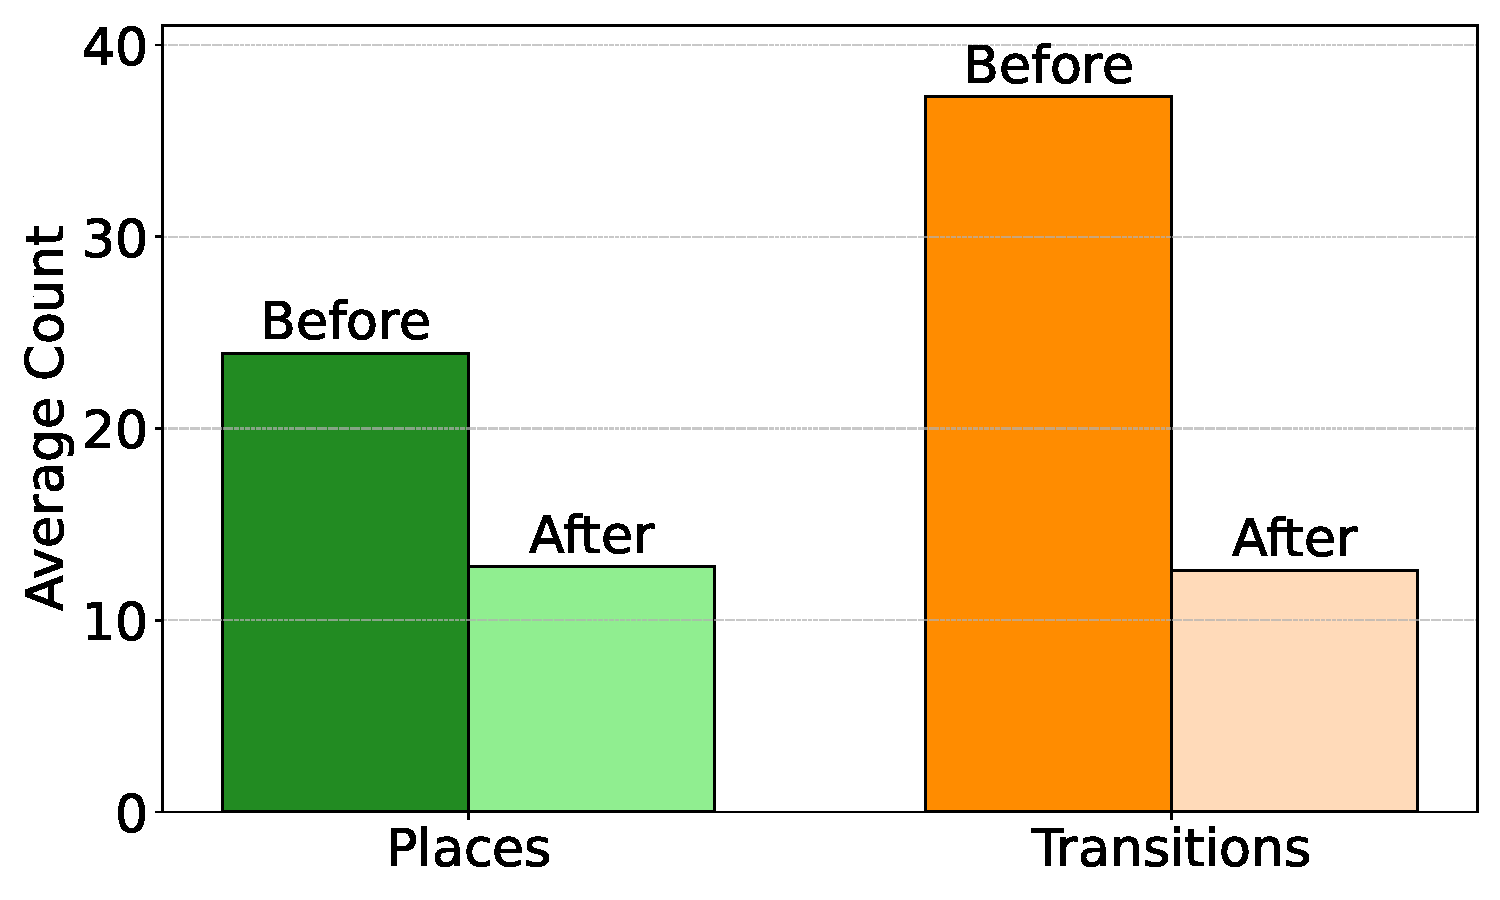
\includegraphics[width=\linewidth]{figures/petri_size_reduction_plot.pdf}
		\captionof{figure}{Reduction of Petri nets size (places and transitions) via bidirectional pruning 
%(timeout 150 seconds)
.}
		\label{fig:petri_size_reduction}
	\end{minipage}
\end{center}







\begin{table}[H]
	\centering
	% Load the tabular from the external file:
	\begin{table}[H]
	\centering
	\begin{tabular}{l c c c c}
		\toprule
		& \multicolumn{2}{c}{number of components} & \multicolumn{2}{c}{periods per component} \\
		\cmidrule(lr){2-3} \cmidrule(lr){4-5}
		& average & max & average & max \\
		\midrule
	all optimizations (baseline) & 2.91 & 22 & 1.33 & 4 \\
	without remove-redundant & 8.79 & 194 & \textbf{1.64} & 11 \\
	without generate-less & \textbf{651.41} & \textbf{20{,}484} & 1.28 & \textbf{15} \\
	without smart-kleene-order & 2.91 & 22 & 1.35 & 4 \\
  \bottomrule
	\end{tabular}
\end{table}

	\caption{Comparison of experiment runs with a 150-second timeout.}
	\label{tab:semilinear-size-reduction}
\end{table}


\newpage





%\section{Comprehensive Statistics}
%\begin{table}[H]
%	\centering
%	\input{tables/comprehensive\_stats.tex}
%	\caption{Comprehensive statistics}
%	\label{tab:comprehensive\_stats}
%\end{table}
%
%\section{Pruning Effectiveness}
%\begin{table}[H]
%	\centering
%	\begin{tabular}{llcccc}
\toprule
Example & Disj. & Places & Transitions & Iter. & Reduction \\n\midrule
\texttt{ex} & 0 & 8 → 8 & 7 → 6 & 2 & 14.3\% \\n\texttt{flag\_non\_ser} & 0 & 9 → 1 & 11 → 0 & 3 & 100.0\% \\n\texttt{flag\_non\_ser} & 1 & 9 → 9 & 11 → 11 & 1 & 0.0\% \\n\texttt{fred\_arith\_tricky2} & 0 & 23 → 15 & 32 → 14 & 2 & 56.2\% \\n\texttt{data\_flow} & 0 & 12 → 9 & 10 → 7 & 2 & 30.0\% \\n\texttt{data\_flow} & 1 & 12 → 9 & 10 → 7 & 2 & 30.0\% \\n\texttt{funny} & 0 & 11 → 11 & 10 → 10 & 1 & 0.0\% \\n\texttt{fred\_arith\_tricky3} & 0 & 36 → 18 & 57 → 19 & 2 & 66.7\% \\n\texttt{login\_flow} & 0 & 17 → 17 & 18 → 18 & 1 & 0.0\% \\n\texttt{login\_flow} & 1 & 17 → 17 & 18 → 18 & 1 & 0.0\% \\n\texttt{state\_machine} & 0 & 17 → 17 & 21 → 18 & 2 & 14.3\% \\n\texttt{state\_machine} & 1 & 17 → 17 & 21 → 18 & 2 & 14.3\% \\n\texttt{modulo\_nonser} & 0 & 11 → 9 & 13 → 11 & 2 & 15.4\% \\n\texttt{fred\_arith\_simplified\_until\_1} & 0 & 14 → 8 & 14 → 6 & 2 & 57.1\% \\n\texttt{fred\_arith\_simplified\_until\_1} & 1 & 14 → 8 & 14 → 6 & 2 & 57.1\% \\n\texttt{fred\_arith\_simplified\_until\_1} & 2 & 14 → 8 & 14 → 6 & 2 & 57.1\% \\n\texttt{fred\_arith\_simplified\_until\_1} & 3 & 14 → 8 & 14 → 6 & 2 & 57.1\% \\n\texttt{fred\_arith\_simplified\_until\_1} & 4 & 14 → 8 & 14 → 6 & 2 & 57.1\% \\n\texttt{fred\_arith\_simplified\_until\_1} & 5 & 14 → 8 & 14 → 6 & 2 & 57.1\% \\n\texttt{nondet} & 0 & 10 → 1 & 15 → 0 & 3 & 100.0\% \\n\texttt{nondet\_impl} & 0 & 24 → 17 & 26 → 16 & 2 & 38.5\% \\n\texttt{multiple\_requests\_updated} & 0 & 17 → 9 & 14 → 8 & 2 & 42.9\% \\n\texttt{multiple\_requests\_updated} & 1 & 17 → 9 & 14 → 8 & 2 & 42.9\% \\n\texttt{nondet2} & 0 & 14 → 14 & 25 → 23 & 2 & 8.0\% \\n\texttt{simple\_nonser2} & 0 & 8 → 8 & 7 → 7 & 1 & 0.0\% \\n\texttt{simple\_nonser2\_turned\_ser\_with\_locks} & 0 & 8 → 8 & 7 → 6 & 2 & 14.3\% \\n\texttt{simple\_nonser} & 0 & 16 → 11 & 18 → 11 & 2 & 38.9\% \\n\texttt{simple\_nonser} & 1 & 16 → 11 & 18 → 11 & 2 & 38.9\% \\n\texttt{simple\_nonser3} & 0 & 8 → 8 & 9 → 9 & 1 & 0.0\% \\n\texttt{fred\_arith\_simplified\_until\_2} & 0 & 19 → 13 & 20 → 10 & 2 & 50.0\% \\n\texttt{fred\_arith\_simplified\_until\_2} & 1 & 19 → 13 & 20 → 10 & 2 & 50.0\% \\n\texttt{fred\_arith\_simplified\_until\_2} & 2 & 19 → 13 & 20 → 10 & 2 & 50.0\% \\n\texttt{fred\_arith\_simplified\_until\_2} & 3 & 19 → 13 & 20 → 10 & 2 & 50.0\% \\n\texttt{fred\_arith\_simplified\_until\_2} & 4 & 19 → 1 & 20 → 0 & 3 & 100.0\% \\n\texttt{fred\_arith\_simplified\_until\_2} & 5 & 19 → 13 & 20 → 10 & 2 & 50.0\% \\n\texttt{fred\_arith\_simplified\_until\_2} & 6 & 19 → 13 & 20 → 10 & 2 & 50.0\% \\n\texttt{fred\_arith\_simplified\_until\_2} & 7 & 19 → 13 & 20 → 10 & 2 & 50.0\% \\n\texttt{fred\_arith\_simplified\_until\_2} & 8 & 19 → 13 & 20 → 10 & 2 & 50.0\% \\n\texttt{fred\_arith\_simplified\_until\_2} & 9 & 19 → 13 & 20 → 10 & 2 & 50.0\% \\n\texttt{fred\_arith\_simplified\_until\_2} & 10 & 19 → 13 & 20 → 10 & 2 & 50.0\% \\n\texttt{fred\_arith\_simplified\_until\_2} & 11 & 19 → 13 & 20 → 10 & 2 & 50.0\% \\n\texttt{fred\_arith\_simplified\_until\_2} & 12 & 19 → 13 & 20 → 10 & 2 & 50.0\% \\n\texttt{shopping\_cart} & 0 & 18 → 16 & 24 → 19 & 2 & 20.8\% \\n\texttt{shopping\_cart} & 1 & 18 → 17 & 24 → 20 & 2 & 16.7\% \\n\texttt{shopping\_cart} & 2 & 18 → 17 & 24 → 20 & 2 & 16.7\% \\n\texttt{shopping\_cart} & 3 & 18 → 18 & 24 → 21 & 2 & 12.5\% \\n\texttt{shopping\_cart} & 4 & 18 → 18 & 24 → 21 & 2 & 12.5\% \\n\texttt{shopping\_cart} & 5 & 18 → 17 & 24 → 20 & 2 & 16.7\% \\n\texttt{incrdecr} & 0 & 21 → 13 & 22 → 10 & 2 & 54.5\% \\n\texttt{incrdecr} & 1 & 21 → 13 & 22 → 10 & 2 & 54.5\% \\n\texttt{incrdecr} & 2 & 21 → 13 & 22 → 10 & 2 & 54.5\% \\n\texttt{incrdecr} & 3 & 21 → 13 & 22 → 10 & 2 & 54.5\% \\n\texttt{incrdecr} & 4 & 21 → 1 & 22 → 0 & 3 & 100.0\% \\n\texttt{incrdecr} & 5 & 21 → 13 & 22 → 10 & 2 & 54.5\% \\n\texttt{incrdecr} & 6 & 21 → 13 & 22 → 10 & 2 & 54.5\% \\n\texttt{incrdecr} & 7 & 21 → 13 & 22 → 10 & 2 & 54.5\% \\n\texttt{incrdecr} & 8 & 21 → 13 & 22 → 10 & 2 & 54.5\% \\n\texttt{incrdecr} & 9 & 21 → 13 & 22 → 10 & 2 & 54.5\% \\n\texttt{incrdecr} & 10 & 21 → 13 & 22 → 10 & 2 & 54.5\% \\n\texttt{incrdecr} & 11 & 21 → 13 & 22 → 10 & 2 & 54.5\% \\n\texttt{incrdecr} & 12 & 21 → 13 & 22 → 10 & 2 & 54.5\% \\n\texttt{nondet\_impl2} & 0 & 24 → 5 & 26 → 4 & 3 & 84.6\% \\n\texttt{nondet\_impl2} & 1 & 24 → 5 & 26 → 4 & 3 & 84.6\% \\n\texttt{nondet\_impl2} & 2 & 24 → 5 & 26 → 4 & 2 & 84.6\% \\n\texttt{nondet\_impl2} & 3 & 24 → 5 & 26 → 4 & 2 & 84.6\% \\n\texttt{nondet\_impl2} & 4 & 24 → 5 & 26 → 4 & 2 & 84.6\% \\n\texttt{modulo} & 0 & 10 → 7 & 10 → 5 & 3 & 50.0\% \\n\texttt{modulo} & 1 & 10 → 10 & 10 → 10 & 1 & 0.0\% \\n\texttt{modulo} & 2 & 10 → 7 & 10 → 5 & 3 & 50.0\% \\n\texttt{modulo} & 3 & 10 → 10 & 10 → 10 & 1 & 0.0\% \\n\texttt{modulo} & 4 & 10 → 10 & 10 → 10 & 1 & 0.0\% \\n\texttt{modulo} & 5 & 10 → 10 & 10 → 10 & 1 & 0.0\% \\n\texttt{modulo} & 6 & 10 → 5 & 10 → 3 & 3 & 70.0\% \\n\texttt{modulo} & 7 & 10 → 7 & 10 → 5 & 3 & 50.0\% \\n\texttt{modulo} & 8 & 10 → 7 & 10 → 5 & 3 & 50.0\% \\n\texttt{modulo} & 9 & 10 → 8 & 10 → 7 & 2 & 30.0\% \\n\texttt{modulo} & 10 & 10 → 10 & 10 → 10 & 1 & 0.0\% \\n\texttt{modulo} & 11 & 10 → 10 & 10 → 10 & 1 & 0.0\% \\n\texttt{modulo} & 12 & 10 → 10 & 10 → 10 & 1 & 0.0\% \\n\texttt{modulo} & 13 & 10 → 8 & 10 → 7 & 2 & 30.0\% \\n\texttt{modulo} & 14 & 10 → 10 & 10 → 10 & 1 & 0.0\% \\n\texttt{modulo} & 15 & 10 → 10 & 10 → 10 & 1 & 0.0\% \\n\texttt{modulo} & 16 & 10 → 10 & 10 → 10 & 1 & 0.0\% \\n\texttt{modulo} & 17 & 10 → 8 & 10 → 7 & 2 & 30.0\% \\n\texttt{modulo} & 18 & 10 → 8 & 10 → 7 & 2 & 30.0\% \\n\texttt{modulo} & 19 & 10 → 10 & 10 → 10 & 1 & 0.0\% \\n\texttt{modulo} & 20 & 10 → 10 & 10 → 10 & 1 & 0.0\% \\n\texttt{snapshot\_isolation\_network\_monitoring} & 0 & 47 → 30 & 94 → 49 & 2 & 47.9\% \\n\texttt{stop3} & 0 & 18 → 18 & 25 → 25 & 1 & 0.0\% \\n\texttt{less\_simple\_ser} & 0 & 30 → 12 & 39 → 14 & 2 & 64.1\% \\n\texttt{less\_simple\_ser} & 1 & 30 → 12 & 39 → 14 & 2 & 64.1\% \\n\texttt{less\_simple\_ser} & 2 & 30 → 12 & 39 → 14 & 2 & 64.1\% \\n\texttt{less\_simple\_ser} & 3 & 30 → 12 & 39 → 14 & 2 & 64.1\% \\n\texttt{less\_simple\_ser} & 4 & 30 → 12 & 39 → 14 & 2 & 64.1\% \\n\texttt{less\_simple\_ser} & 5 & 30 → 12 & 39 → 14 & 2 & 64.1\% \\n\texttt{less\_simple\_ser} & 6 & 30 → 4 & 39 → 3 & 3 & 92.3\% \\n\texttt{less\_simple\_ser} & 7 & 30 → 4 & 39 → 3 & 3 & 92.3\% \\n\texttt{less\_simple\_ser} & 8 & 30 → 4 & 39 → 3 & 3 & 92.3\% \\n\texttt{stop2} & 0 & 14 → 14 & 19 → 13 & 2 & 31.6\% \\n\texttt{stop2} & 1 & 14 → 11 & 19 → 11 & 2 & 42.1\% \\n\texttt{stop2} & 2 & 14 → 8 & 19 → 6 & 2 & 68.4\% \\n\texttt{stop2} & 3 & 14 → 11 & 19 → 8 & 2 & 57.9\% \\n\texttt{stop2} & 4 & 14 → 11 & 19 → 8 & 2 & 57.9\% \\n\texttt{stop2} & 5 & 14 → 14 & 19 → 13 & 2 & 31.6\% \\n\texttt{stop2} & 6 & 14 → 11 & 19 → 11 & 2 & 42.1\% \\n\texttt{stateful\_firewall} & 0 & 22 → 1 & 24 → 0 & 3 & 100.0\% \\n\texttt{stateful\_firewall} & 1 & 22 → 1 & 24 → 0 & 3 & 100.0\% \\n\texttt{stateful\_firewall} & 2 & 22 → 1 & 24 → 0 & 3 & 100.0\% \\n\texttt{stateful\_firewall} & 3 & 22 → 15 & 24 → 15 & 3 & 37.5\% \\n\texttt{stateful\_firewall} & 4 & 22 → 10 & 24 → 10 & 3 & 58.3\% \\n\texttt{stateful\_firewall} & 5 & 22 → 10 & 24 → 10 & 3 & 58.3\% \\n\texttt{stateful\_firewall} & 6 & 22 → 15 & 24 → 15 & 3 & 37.5\% \\n\texttt{stateful\_firewall} & 7 & 22 → 15 & 24 → 15 & 3 & 37.5\% \\n\texttt{stateful\_firewall} & 8 & 22 → 17 & 24 → 18 & 3 & 25.0\% \\n\texttt{stateful\_firewall} & 9 & 22 → 1 & 24 → 0 & 3 & 100.0\% \\n\texttt{stateful\_firewall} & 10 & 22 → 17 & 24 → 18 & 3 & 25.0\% \\n\texttt{stateful\_firewall} & 11 & 22 → 17 & 24 → 18 & 3 & 25.0\% \\n\texttt{stateful\_firewall} & 12 & 22 → 15 & 24 → 16 & 3 & 33.3\% \\n\texttt{stateful\_firewall} & 13 & 22 → 19 & 24 → 20 & 3 & 16.7\% \\n\texttt{stateful\_firewall} & 14 & 22 → 17 & 24 → 17 & 3 & 29.2\% \\n\texttt{stateful\_firewall} & 15 & 22 → 5 & 24 → 3 & 3 & 87.5\% \\n\texttt{stateful\_firewall} & 16 & 22 → 5 & 24 → 3 & 3 & 87.5\% \\n\texttt{stateful\_firewall} & 17 & 22 → 5 & 24 → 3 & 3 & 87.5\% \\n\texttt{stateful\_firewall} & 18 & 22 → 19 & 24 → 20 & 3 & 16.7\% \\n\texttt{stateful\_firewall} & 19 & 22 → 19 & 24 → 20 & 3 & 16.7\% \\n\texttt{stateful\_firewall} & 20 & 22 → 10 & 24 → 7 & 3 & 70.8\% \\n\texttt{stateful\_firewall} & 21 & 22 → 10 & 24 → 7 & 3 & 70.8\% \\n\texttt{stateful\_firewall} & 22 & 22 → 22 & 24 → 24 & 1 & 0.0\% \\n\texttt{stateful\_firewall} & 23 & 22 → 20 & 24 → 22 & 2 & 8.3\% \\n\texttt{snapshot\_isolation\_network\_monitoring\_without\_yields} & 0 & 26 → 16 & 34 → 17 & 2 & 50.0\% \\n\texttt{snapshot\_isolation\_network\_monitoring\_without\_yields} & 1 & 26 → 16 & 34 → 17 & 2 & 50.0\% \\n\texttt{snapshot\_isolation\_network\_monitoring\_without\_yields} & 2 & 26 → 1 & 34 → 0 & 3 & 100.0\% \\n\texttt{snapshot\_isolation\_network\_monitoring\_without\_yields} & 3 & 26 → 1 & 34 → 0 & 3 & 100.0\% \\n\texttt{snapshot\_isolation\_network\_monitoring\_without\_yields} & 4 & 26 → 1 & 34 → 0 & 3 & 100.0\% \\n\texttt{snapshot\_isolation\_network\_monitoring\_without\_yields} & 5 & 26 → 16 & 34 → 17 & 2 & 50.0\% \\n\texttt{BGP\_routing} & 0 & 101 → 39 & 159 → 55 & 2 & 65.4\% \\n\texttt{BGP\_routing} & 1 & 101 → 39 & 159 → 55 & 2 & 65.4\% \\n\texttt{complex\_while\_with\_yields} & 0 & 34 → 18 & 48 → 17 & 2 & 64.6\% \\n\texttt{stop4} & 0 & 18 → 15 & 25 → 11 & 2 & 56.0\% \\n\texttt{stop4} & 1 & 18 → 9 & 25 → 7 & 2 & 72.0\% \\n\texttt{stop4} & 2 & 18 → 12 & 25 → 9 & 2 & 64.0\% \\n\texttt{stop4} & 3 & 18 → 12 & 25 → 9 & 2 & 64.0\% \\n\texttt{stop4} & 4 & 18 → 18 & 25 → 17 & 2 & 32.0\% \\n\texttt{stop4} & 5 & 18 → 15 & 25 → 15 & 2 & 40.0\% \\n\texttt{stop4} & 6 & 18 → 12 & 25 → 13 & 2 & 48.0\% \\n\texttt{fred\_arith\_tricky} & 0 & 29 → 17 & 46 → 22 & 2 & 52.2\% \\n\texttt{fred2\_arith} & 0 & 40 → 24 & 78 → 38 & 2 & 51.3\% \\n\texttt{bank\_without\_yields} & 0 & 69 → 37 & 135 → 48 & 2 & 64.4\% \\n\texttt{bank\_without\_yields} & 1 & 69 → 37 & 135 → 48 & 2 & 64.4\% \\n\texttt{tricky2} & 0 & 65 → 25 & 99 → 35 & 2 & 64.6\% \\n\texttt{tricky2} & 1 & 65 → 25 & 99 → 35 & 2 & 64.6\% \\n\texttt{tricky2} & 2 & 65 → 25 & 99 → 35 & 2 & 64.6\% \\n\texttt{stop} & 0 & 14 → 11 & 19 → 15 & 3 & 21.1\% \\n\texttt{stop} & 1 & 14 → 8 & 19 → 7 & 3 & 63.2\% \\n\texttt{stop4a} & 0 & 18 → 18 & 25 → 17 & 2 & 32.0\% \\n\texttt{stop4a} & 1 & 18 → 12 & 25 → 13 & 2 & 48.0\% \\n\texttt{stop4a} & 2 & 18 → 15 & 25 → 15 & 2 & 40.0\% \\n\texttt{stop4a} & 3 & 18 → 15 & 25 → 15 & 2 & 40.0\% \\n\texttt{stop4a} & 4 & 18 → 12 & 25 → 9 & 2 & 64.0\% \\n\texttt{stop4a} & 5 & 18 → 9 & 25 → 7 & 2 & 72.0\% \\n\texttt{stop4a} & 6 & 18 → 15 & 25 → 11 & 2 & 56.0\% \\n\texttt{stop4a} & 7 & 18 → 15 & 25 → 11 & 2 & 56.0\% \\n\texttt{stop4a} & 8 & 18 → 12 & 25 → 9 & 2 & 64.0\% \\n\texttt{stop4a} & 9 & 18 → 18 & 25 → 17 & 2 & 32.0\% \\n\texttt{stop4a} & 10 & 18 → 15 & 25 → 15 & 2 & 40.0\% \\n\texttt{stop4a} & 11 & 18 → 12 & 25 → 13 & 2 & 48.0\% \\n\texttt{stop4a} & 12 & 18 → 18 & 25 → 17 & 2 & 32.0\% \\n\texttt{stop4a} & 13 & 18 → 15 & 25 → 15 & 2 & 40.0\% \\n\texttt{stop4a} & 14 & 18 → 12 & 25 → 13 & 2 & 48.0\% \\n\texttt{stop3a} & 0 & 18 → 12 & 25 → 17 & 3 & 32.0\% \\n\texttt{stop3a} & 1 & 18 → 12 & 25 → 17 & 3 & 32.0\% \\n\texttt{tricky3} & 0 & 77 → 29 & 123 → 43 & 2 & 65.0\% \\n\texttt{tricky3} & 1 & 77 → 29 & 123 → 43 & 2 & 65.0\% \\n\texttt{tricky3} & 2 & 77 → 29 & 123 → 43 & 2 & 65.0\% \\n\texttt{bank} & 0 & 86 → 56 & 285 → 103 & 2 & 63.9\% \\n\texttt{tricky3\_ser} & 0 & 78 → 8 & 174 → 7 & 3 & 96.0\% \\n\texttt{tricky3\_ser} & 1 & 78 → 8 & 174 → 7 & 3 & 96.0\% \\n\texttt{tricky3\_ser} & 2 & 78 → 8 & 174 → 7 & 3 & 96.0\% \\n\texttt{tricky3\_ser} & 3 & 78 → 17 & 174 → 20 & 3 & 88.5\% \\n\texttt{tricky3\_ser} & 4 & 78 → 17 & 174 → 20 & 3 & 88.5\% \\n\texttt{tricky3\_ser} & 5 & 78 → 34 & 174 → 62 & 2 & 64.4\% \\n\texttt{tricky3\_ser} & 6 & 78 → 34 & 174 → 62 & 2 & 64.4\% \\n\texttt{tricky3\_ser} & 7 & 78 → 31 & 174 → 43 & 3 & 75.3\% \\n\bottomrule
\end{tabular}

%	\caption{Petri net pruning effectiveness}
%	\label{tab:pruning\_effectiveness}
%\end{table}
%
%\section{Timing Comparison}
%\begin{table}[H]
%	\centering
%	\begin{tabular}{lccccc}
\toprule
Example & Unopt. & Opt. & Speedup & Create & Check \\
\midrule
\texttt{bank_without_yields} & 48.0s & 41.9s & 1.1× & 32.4s & 0ms \\
\texttt{complex_while_with_yields} & 43.4s & 40.9s & 1.1× & 30.3s & 0ms \\
\texttt{data_flow} & 8.3s & 5.8s & 1.4× & 812ms & 1.1s \\
\texttt{ex} & 3.2s & 3.3s & 1.0× & 430ms & 97ms \\
\texttt{flag_non_ser} & 32.6s & 3.4s & 9.6× & 865ms & 0ms \\
\texttt{flag_non_ser_turned_ser} & 2.3s & 2.7s & 0.8× & 4ms & 13ms \\
\texttt{fred2_arith} & 41.5s & 38.7s & 1.1× & 30.3s & 0ms \\
\texttt{fred_arith_simplified_until_1} & 32.3s & 15.1s & 2.1× & 2.0s & 5.1s \\
\texttt{fred_arith_tricky} & 35.3s & 33.5s & 1.1× & 29.4s & 0ms \\
\texttt{fred_arith_tricky2} & 5.1s & 4.2s & 1.2× & 407ms & 0ms \\
\texttt{fred_arith_tricky3} & 9.0s & 6.4s & 1.4× & 607ms & 0ms \\
\texttt{funny} & 2.6s & 2.5s & 1.0× & 314ms & 0ms \\
\texttt{if_while_with_req} & 2.1s & 2.0s & 1.0× & 1ms & 3ms \\
\texttt{login_flow} & 29.8s & 23.0s & 1.3× & 821ms & 10.3s \\
\texttt{modulo} & 55.6s & 35.5s & 1.6× & 5.8s & 12.9s \\
\texttt{modulo_nonser} & 6.9s & 2.7s & 2.5× & 472ms & 0ms \\
\texttt{multiple_requests_updated} & 11.6s & 6.1s & 1.9× & 523ms & 1.5s \\
\texttt{nested_while} & 2.1s & 2.1s & 1.0× & 1ms & 1ms \\
\texttt{nondet} & 5.4s & 2.6s & 2.1× & 273ms & 38ms \\
\texttt{nondet2} & 4.7s & 3.2s & 1.5× & 508ms & 0ms \\
\texttt{nondet_impl} & 2.9s & 2.5s & 1.2× & 350ms & 0ms \\
\texttt{nondet_impl2} & 43.7s & 47.7s & 0.9× & 1.2s & 22.0s \\
\texttt{self_loop} & 2.2s & 1.9s & 1.1× & 1ms & 2ms \\
\texttt{self_loop2} & 4.0s & 2.8s & 1.5× & 4ms & 14ms \\
\texttt{simple_nonser} & 2.6s & 2.4s & 1.1× & 544ms & 0ms \\
\texttt{simple_nonser2} & 2.2s & 2.2s & 1.0× & 320ms & 0ms \\
\texttt{simple_nonser2_minus_yields_is_ser} & 1.9s & 1.7s & 1.1× & 1ms & 2ms \\
\texttt{simple_nonser2_turned_ser_with_locks} & 2.6s & 2.8s & 0.9× & 448ms & 107ms \\
\texttt{simple_nonser3} & 2.5s & 2.7s & 0.9× & 371ms & 0ms \\
\texttt{snapshot_isolation_network_monitoring} & 28.1s & 17.3s & 1.6× & 4.0s & 0ms \\
\texttt{state_machine} & 35.3s & 25.1s & 1.4× & 848ms & 11.3s \\
\texttt{stateful_firewall} & 10.8s & 9.5s & 1.1× & 6.6s & 0ms \\
\texttt{stop} & 34.2s & 33.4s & 1.0× & 30.5s & 0ms \\
\texttt{stop2} & 59.3s & 29.8s & 2.0× & 1.7s & 12.3s \\
\texttt{stop3} & 5.6s & 3.8s & 1.5× & 358ms & 0ms \\
\texttt{stop3a} & 36.1s & 33.9s & 1.1× & 30.5s & 0ms \\
\texttt{tricky2} & 46.4s & 40.6s & 1.1× & 29.3s & 0ms \\
\texttt{tricky3} & 58.6s & 52.2s & 1.1× & 31.0s & 0ms \\
\bottomrule
\end{tabular}

%	\caption{Comparison of optimized vs.\ unoptimized run times}
%	\label{tab:timing\_comparison}
%\end{table}
%
%\section{Optimization Breakdown}
%\begin{table}[H]
%	\centering
%	\begin{tabular}{lcccccc}
\toprule
Example & No Opt & B & R & G & S & All Opt \\
\midrule
\texttt{data_flow} & 4.1s & 7.3s & -- & -- & 9.3s & 6.6s \\
\texttt{ex} & 2.4s & 3.3s & 4.2s & 5.2s & 3.5s & 2.7s \\
\texttt{flag_non_ser} & 7.1s & 3.4s & 8.7s & 8.8s & 8.2s & 3.1s \\
\texttt{flag_non_ser_turned_ser} & 1.9s & 2.8s & 2.9s & 3.8s & 2.6s & 2.5s \\
\texttt{fred_arith_tricky} & 8.4s & -- & -- & -- & -- & 8.1s \\
\texttt{fred_arith_tricky2} & 3.7s & 6.1s & 6.6s & 7.7s & 7.2s & 4.8s \\
\texttt{fred_arith_tricky3} & 5.2s & -- & -- & -- & -- & 9.5s \\
\texttt{funny} & 2.7s & 3.1s & 2.6s & 4.1s & 2.7s & 2.7s \\
\texttt{if_while_with_req} & 2.6s & 2.2s & 2.0s & 2.9s & 2.1s & 1.7s \\
\texttt{nested_while} & 2.0s & 2.4s & 2.5s & 2.6s & 2.4s & 1.8s \\
\texttt{nondet} & 5.1s & 5.4s & 9.6s & -- & 9.1s & 3.7s \\
\texttt{nondet2} & 4.7s & 7.6s & 8.0s & 8.3s & 7.2s & 6.8s \\
\texttt{nondet_impl} & 2.9s & 4.6s & 4.8s & 5.5s & 5.1s & 3.0s \\
\texttt{self_loop} & 2.0s & 2.4s & 2.4s & 3.2s & 3.1s & 2.3s \\
\texttt{self_loop2} & 3.5s & 6.6s & 6.9s & 6.4s & 6.4s & 5.7s \\
\texttt{simple_nonser} & 3.0s & 4.2s & 4.7s & 4.0s & 4.1s & 4.1s \\
\texttt{simple_nonser2} & 2.9s & 3.7s & 4.0s & 3.4s & 3.6s & 3.9s \\
\texttt{simple_nonser2_minus_yields_is_ser} & 2.4s & 3.1s & 3.6s & 2.7s & 2.4s & 3.5s \\
\texttt{simple_nonser2_turned_ser_with_locks} & 2.9s & 4.5s & 4.5s & 4.1s & 3.7s & 4.2s \\
\texttt{simple_nonser3} & 2.6s & 3.8s & 4.3s & 3.6s & 3.1s & 3.7s \\
\texttt{stop} & 8.8s & -- & -- & -- & -- & 9.5s \\
\texttt{stop3} & 5.4s & 7.2s & 8.2s & 7.4s & 7.2s & 5.4s \\
\bottomrule
\end{tabular}

% B = Bidirectional Pruning, R = Remove Redundant, G = Generate Less, S = Smart Kleene Order

%	\caption{Impact of individual optimizations}
%	\label{tab:optimization\_breakdown}
%\end{table}
%
%\section{Summary Statistics}
%\begin{table}[H]
%	\centering
%	\begin{itemize}
\item Total examples analyzed: 40
\item Serializable: 18 (45.0\%)
\item Not serializable: 16 (40.0\%)
\item Timeouts: 6 (15.0\%)
\item Average pruning effectiveness: 119.3\%
\item Average analysis time: 17.1s
\end{itemize}

%	\caption{Overall summary statistics}
%	\label{tab:summary\_stats}
%\end{table}